\documentclass[journal]{IEEEtran}
\usepackage{cite}
\usepackage{amsmath,amssymb,amsfonts}
\usepackage{algorithmic}
\usepackage{graphicx}
\usepackage{textcomp}
\usepackage{xcolor}
\usepackage{url}
\usepackage{hyperref}
\usepackage{tikz}
\usetikzlibrary{shapes.geometric, arrows.meta, positioning, fit, backgrounds, calc}

\begin{document}

\title{Robot Zombie Apocalypse: Security Implications of Wormable Exploits in Autonomous Robotics and IoT Infrastructure}

\author{Ezekiel Ologunde%
\thanks{}}

\markboth{Robotics and Automation Security, October 2025}%
{Ologunde: Robot Zombie Apocalypse}

\maketitle

\begin{abstract}
The convergence of robotics, Internet of Things (IoT), and autonomous systems introduces
unprecedented security challenges. This paper examines the UniPwn exploit affecting
Unitree robotic platforms, which demonstrates the catastrophic potential of wormable
vulnerabilities in autonomous systems. Through analysis of the exploit chain---comprising
hardcoded cryptographic keys, insufficient handshake verification, and unsafe input
handling---we reveal how attackers achieve root-level privilege escalation and establish
autonomous robot-to-robot propagation. The wormable nature enables compromised robots to
autonomously infect nearby devices over wireless protocols, creating what security
researchers term a ``robot zombie apocalypse'' scenario. For critical infrastructure
applications employing autonomous inspection robots, drones, and unmanned vehicles, these
vulnerabilities present existential risks enabling adversaries to weaponize trusted
automation systems against the infrastructure they were designed to protect. We propose a
seven-layer defense-in-depth security framework addressing firmware security, wireless
protocol hardening, physical-cyber boundary protection, and strategies specific to
autonomous robotic systems.
\end{abstract}

\begin{IEEEkeywords}
Robotics security, IoT vulnerabilities, wormable exploits, autonomous systems, wireless
security, firmware security, critical infrastructure, UniPwn, robot-to-robot propagation
\end{IEEEkeywords}

\section{Introduction}
\IEEEPARstart{T}{he} rapid proliferation of autonomous robotic systems and IoT devices
across industrial, commercial, and critical infrastructure environments introduces
security challenges fundamentally different from traditional IT threats. The discovery of
the UniPwn exploit in October 2025, affecting Unitree's humanoid and quadrupedal robot
platforms, exemplifies the catastrophic potential when these unique challenges
converge~\cite{udinmwen2025calm}.

UniPwn enables complete remote control of affected robots and autonomous propagation to
nearby devices without continued attacker involvement. Security researchers have described
potential outcomes as a ``robot zombie apocalypse''---terminology that accurately captures
the autonomous, self-propagating nature of the threat~\cite{naraine2025hackers}. Unitree
robots have been adopted for pipeline monitoring, electrical transmission line inspection,
and perimeter security~\cite{gosavi2025unitree}; when compromised and weaponized, the
consequences escalate from information security incidents to physical safety crises.

\subsection{The UniPwn Vulnerability Chain}

The exploit chains four components: (1)~\textbf{hardcoded keys} identical across all
units enabling any extracted key to attack all similar devices globally;
(2)~\textbf{insufficient handshake verification} permitting authenticated sessions without
proper credential validation; (3)~\textbf{unsafe input handling} enabling command
injection to root privilege~\cite{udinmwen2025calm}; and (4)~\textbf{wireless propagation}
allowing compromised robots to autonomously scan, connect, and exploit nearby Unitree
devices via Bluetooth and Wi-Fi. Additionally, researchers found telemetry transmitted to
servers in China every five minutes~\cite{gosavi2025unitree}.

\subsection{Research Contributions}

This paper: (1)~provides comprehensive analysis of the UniPwn exploit chain;
(2)~examines wormable exploit propagation dynamics; (3)~analyzes wireless vulnerabilities
bypassing perimeter defenses; (4)~assesses critical infrastructure implications; and
(5)~proposes a seven-layer defense framework.

\section{Background and Related Work}

\subsection{IoT and Robotics Security}

The 2016 Mirai botnet demonstrated IoT vulnerability at scale~\cite{antonakakis2017understanding}
but targeted stationary devices. Robotic systems add physical actuators enabling kinetic
effects, mobility traversing restricted areas, complex sensor suites enabling espionage,
and resource constraints limiting security mechanisms.

\subsection{Wormable Exploits}

Wormable vulnerabilities---enabling autonomous propagation without user
interaction---represent severe threats, as demonstrated by Morris Worm, Code Red, and
WannaCry~\cite{weaver2003very}. UniPwn represents an evolution: wormable exploitation of
physically mobile, wirelessly connected devices. Proximity-based propagation creates
localized infection clusters; physical mobility enables crossing network segments; diverse
wireless protocols provide multiple propagation vectors; and disruption extends beyond
information theft to kinetic effects.

\subsection{Firmware Security}

Hardcoded credentials and weak cryptographic implementations remain widespread despite
decades of research~\cite{costin2014large}, driven by legacy design assumptions of
physical isolation, resource constraints, update operational complexity, and fragmented
supply chain security responsibility.

\begin{figure}[!t]
\centering
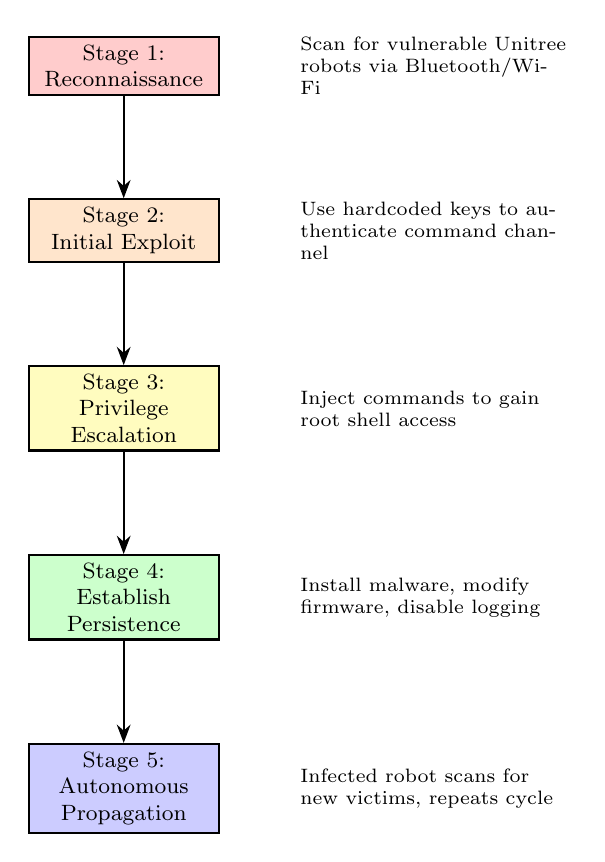
\begin{tikzpicture}[
  node distance=1.3cm,
  font=\footnotesize,
  >=Stealth,
  box/.style={rectangle, draw, thick, minimum width=2.4cm, minimum height=0.72cm,
              align=center, text width=2.2cm, inner sep=3pt},
  arr/.style={-{Stealth}, thick}
]
  \node[box, fill=red!20]    (recon)    {Stage 1:\\Reconnaissance};
  \node[box, fill=orange!20, below=of recon]   (exploit)  {Stage 2:\\Initial Exploit};
  \node[box, fill=yellow!25, below=of exploit] (escalate) {Stage 3:\\Privilege Escalation};
  \node[box, fill=green!20,  below=of escalate](persist)  {Stage 4:\\Establish Persistence};
  \node[box, fill=blue!20,   below=of persist] (propagate){Stage 5:\\Autonomous Propagation};
  \draw[arr] (recon)--(exploit); \draw[arr] (exploit)--(escalate);
  \draw[arr] (escalate)--(persist); \draw[arr] (persist)--(propagate);
  \node[right=0.9cm of recon,   text width=3.4cm, font=\scriptsize, align=left]
    {Scan for vulnerable Unitree robots via Bluetooth/Wi-Fi};
  \node[right=0.9cm of exploit, text width=3.4cm, font=\scriptsize, align=left]
    {Use hardcoded keys to authenticate command channel};
  \node[right=0.9cm of escalate,text width=3.4cm, font=\scriptsize, align=left]
    {Inject commands to gain root shell access};
  \node[right=0.9cm of persist, text width=3.4cm, font=\scriptsize, align=left]
    {Install malware, modify firmware, disable logging};
  \node[right=0.9cm of propagate,text width=3.4cm, font=\scriptsize, align=left]
    {Infected robot scans for new victims, repeats cycle};
\end{tikzpicture}
\caption{UniPwn exploit chain: five-stage attack progression from reconnaissance
  through autonomous propagation, exploiting hardcoded keys, insufficient authentication,
  and unsafe input handling.}
\label{fig:exploit_chain}
\end{figure}

\subsection{Critical Infrastructure Applications}

Autonomous robots are deployed in pipeline inspection, electrical infrastructure
monitoring, perimeter security, and hazardous environment operations~\cite{murphy2019robotics}.
Compromise enabling false ``all clear'' inspection reports could mask failures leading to
environmental disaster; weaponized security robots could facilitate physical intrusions
or harm personnel.

\section{UniPwn Threat Analysis}

\subsection{Vulnerability Technical Details}

\textbf{Hardcoded Keys (CWE-798)}: Keys embedded in firmware are identical across all
units; any extracted key attacks all similar devices globally. Proper practice requires
per-device key provisioning during manufacturing, hardware security modules for storage,
and key derivation functions generating session-specific keys~\cite{naraine2025hackers}.

\textbf{Insufficient Authentication (CWE-287)}: The handshake accepts any client
presenting hardcoded keys with no additional factor, no device certificate validation, and
no anomaly detection. Secure practice requires PKI with per-device certificates,
challenge-response protocols, time-limited session tokens, and rate limiting.

\textbf{Command Injection (CWE-77, CWE-78)}: Authenticated commands are passed to system
functions without sanitization~\cite{udinmwen2025calm}, enabling privilege escalation to
root, persistent backdoor installation, and firmware modification. Mitigation requires
whitelist input validation, parameterized commands, and least-privilege execution.

\textbf{Autonomous Propagation}: Once compromised, the malware scans for
Bluetooth/Wi-Fi devices advertising Unitree service identifiers, initiates connections
using hardcoded keys, executes the full exploit chain automatically, installs the
propagation payload, and each newly compromised robot begins scanning for additional
victims---creating exponential propagation within multi-robot environments.

\begin{figure*}[!t]
\centering
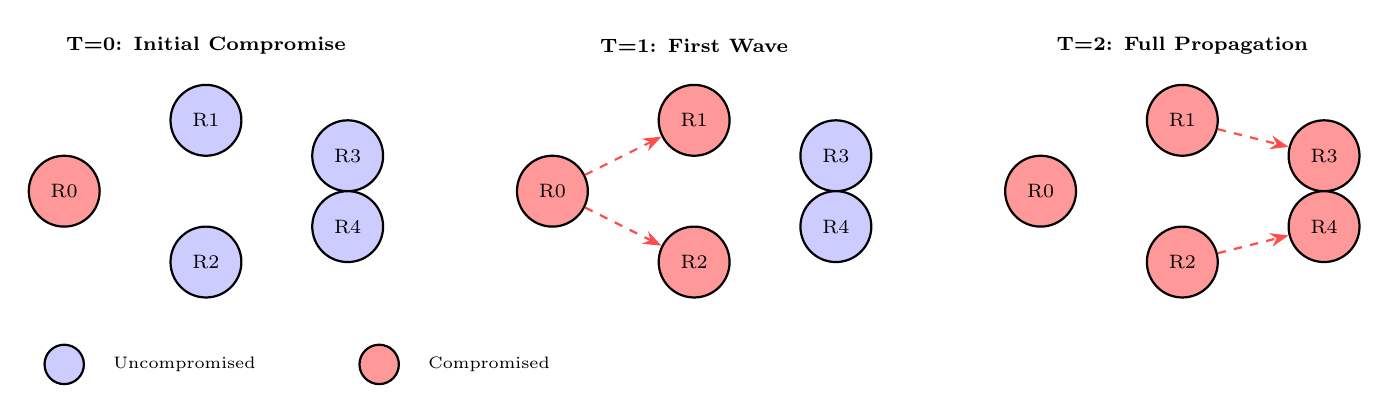
\begin{tikzpicture}[
  font=\fontsize{7pt}{9pt}\selectfont,
  >=Stealth,
  bot/.style={circle, draw, thick, minimum size=0.9cm,
              fill=blue!20, text centered},
  bad/.style={circle, draw, thick, minimum size=0.9cm,
              fill=red!40, text centered},
  arr/.style={-{Stealth}, thick, red!70, dashed}
]

  %%── Helper: draw one panel ──────────────────────────────────────────────
  %% Panel origin at (ox, 0). Nodes at offsets below.

  %% ── T=0  (ox = 0) ────────────────────────────────────────────────────
  \def\ox{0}
  \node[bad] (a0) at (\ox+0, 0)    {R0};
  \node[bot] (a1) at (\ox+1.8, 0.9)  {R1};
  \node[bot] (a2) at (\ox+1.8,-0.9)  {R2};
  \node[bot] (a3) at (\ox+3.6, 0.45) {R3};
  \node[bot] (a4) at (\ox+3.6,-0.45) {R4};
  \node[font=\fontsize{7pt}{9pt}\selectfont\bfseries]
    at (\ox+1.8, 1.85) {T=0: Initial Compromise};

  %% ── T=1  (ox = 6.2) ──────────────────────────────────────────────────
  \def\ox{6.2}
  \node[bad] (b0) at (\ox+0, 0)      {R0};
  \node[bad] (b1) at (\ox+1.8, 0.9)  {R1};
  \node[bad] (b2) at (\ox+1.8,-0.9)  {R2};
  \node[bot] (b3) at (\ox+3.6, 0.45) {R3};
  \node[bot] (b4) at (\ox+3.6,-0.45) {R4};
  \node[font=\fontsize{7pt}{9pt}\selectfont\bfseries]
    at (\ox+1.8, 1.85) {T=1: First Wave};
  \draw[arr] (b0) -- (b1);
  \draw[arr] (b0) -- (b2);

  %% ── T=2  (ox = 12.4) ─────────────────────────────────────────────────
  \def\ox{12.4}
  \node[bad] (c0) at (\ox+0, 0)      {R0};
  \node[bad] (c1) at (\ox+1.8, 0.9)  {R1};
  \node[bad] (c2) at (\ox+1.8,-0.9)  {R2};
  \node[bad] (c3) at (\ox+3.6, 0.45) {R3};
  \node[bad] (c4) at (\ox+3.6,-0.45) {R4};
  \node[font=\fontsize{7pt}{9pt}\selectfont\bfseries]
    at (\ox+1.8, 1.85) {T=2: Full Propagation};
  \draw[arr] (c1) -- (c3);
  \draw[arr] (c2) -- (c4);

  %% ── Legend ───────────────────────────────────────────────────────────
  \node[bot, minimum size=0.5cm] at (0.0,-2.2) {};
  \node[anchor=west, font=\fontsize{6.5pt}{8pt}\selectfont]
    at (0.5,-2.2) {Uncompromised};
  \node[bad, minimum size=0.5cm] at (4.0,-2.2) {};
  \node[anchor=west, font=\fontsize{6.5pt}{8pt}\selectfont]
    at (4.5,-2.2) {Compromised};

\end{tikzpicture}
\caption{Autonomous propagation dynamics of the UniPwn worm: single compromised
  robot R0 spreads to R1 and R2 in the first wave, then R1 and R2 each infect
  further robots until all five are compromised. Blue circles are uninfected;
  red circles are compromised. Dashed arrows show wireless propagation vectors.}
\label{fig:propagation}
\end{figure*}

\subsection{Attack Scenarios}

\textbf{Pipeline Sabotage}: An adversary compromises a single inspection robot, causes
it to report false ``all clear'' results, propagates to the entire fleet via worm, and
either masks pipeline damage until catastrophic failure or commands physical sabotage.

\textbf{Facility Security}: A compromised security robot disables intrusion detection,
propagates to other security units, enables adversary camera/LIDAR exfiltration, and
opens access control points to facilitate unauthorized entry.

\textbf{Warehouse Disruption}: Ransomware operators compromise warehouse robots; at a
coordinated trigger time all robots simultaneously cease operations and display ransom
demands.

\section{Unique Security Challenges in Robotic Systems}

\subsection{Wireless Communication as Attack Surface}

Robots incorporate Wi-Fi, Bluetooth/BLE, cellular, and proprietary RF interfaces that
bypass conventional perimeter defenses entirely~\cite{udinmwen2025calm}. An adversary
within wireless range can attempt exploitation without traversing any firewall.
Robot-to-robot propagation over direct wireless links is invisible to conventional
north-south network monitoring.

\subsection{Firmware and Update Challenges}

Proper remediation of hardcoded keys approaches a complete system redesign, requiring
per-device identity generation, HSM deployment, key management infrastructure, and
protocol redesign. Mixed fleets including legacy robots without HSM or TEE capabilities
face difficult replace-or-accept-risk decisions.

\subsection{Physical-Cyber Boundary}

Compromised robots can cause physical damage through actuator control, be misdirected via
sensor spoofing (GPS, LIDAR, camera injection), disable safety interlocks, and manipulate
facility access control. Unitree humanoid robots possess articulated manipulators capable
of grasping objects and opening doors---kinetic threat potential absent in traditional
malware.

\begin{figure*}[!t]
\centering
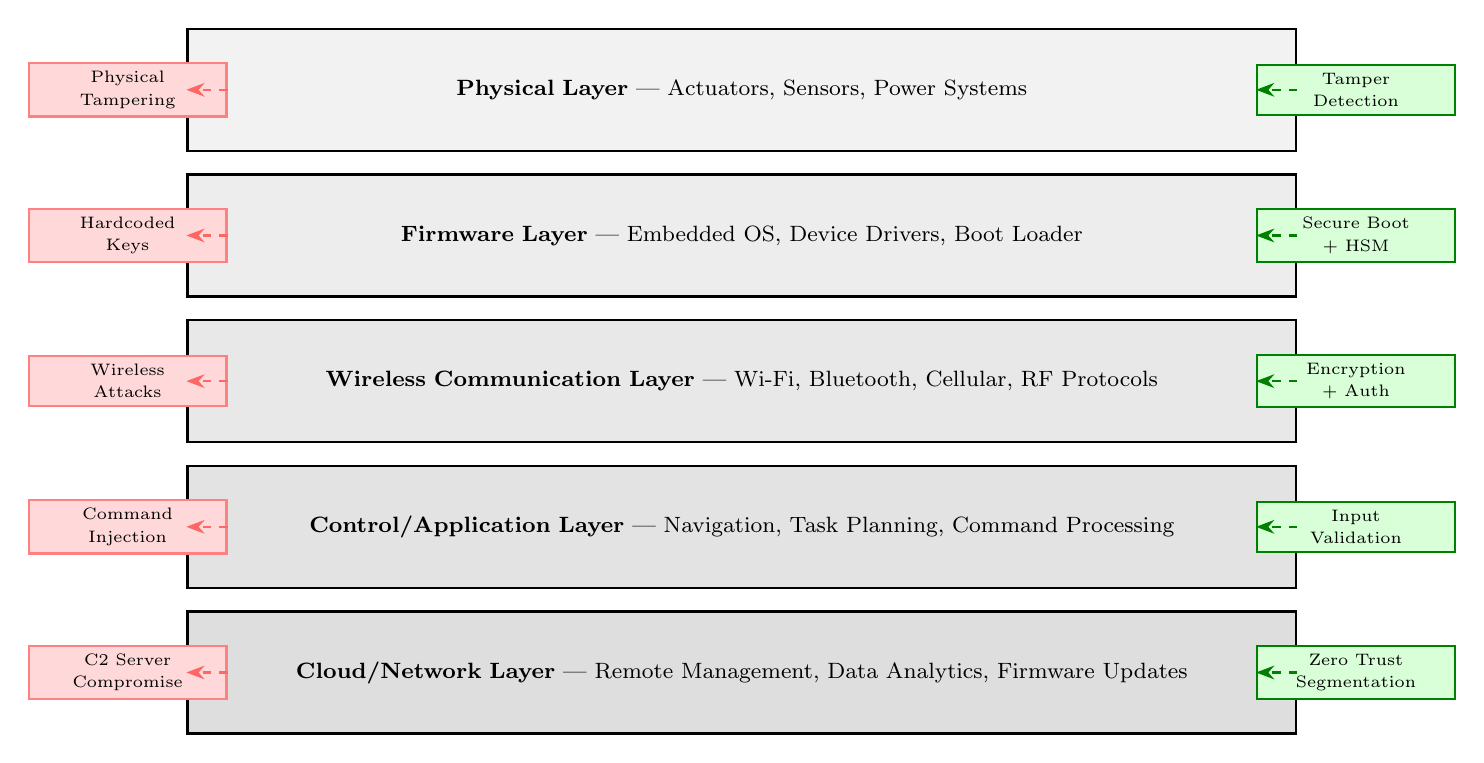
\begin{tikzpicture}[
  font=\footnotesize,
  >=Stealth,
  lyr/.style={rectangle, draw, thick, minimum width=14.0cm, minimum height=1.55cm,
              align=center, text width=13.8cm, inner sep=4pt},
  thr/.style={rectangle, draw=red!50, fill=red!15, thick,
              minimum width=2.5cm, minimum height=0.58cm,
              align=center, font=\fontsize{6.5pt}{8pt}\selectfont,
              text width=2.3cm, inner sep=3pt},
  ctr/.style={rectangle, draw=green!50!black, fill=green!15, thick,
              minimum width=2.5cm, minimum height=0.58cm,
              align=center, font=\fontsize{6.5pt}{8pt}\selectfont,
              text width=2.3cm, inner sep=3pt},
  arr/.style={-{Stealth}, thick, dashed}
]
  \node[lyr, fill=gray!10] (phy)  at (0, 0.00) {\textbf{Physical Layer} --- Actuators, Sensors, Power Systems};
  \node[lyr, fill=gray!14] (fw)   at (0,-1.85) {\textbf{Firmware Layer} --- Embedded OS, Device Drivers, Boot Loader};
  \node[lyr, fill=gray!18] (wl)   at (0,-3.70) {\textbf{Wireless Communication Layer} --- Wi-Fi, Bluetooth, Cellular, RF Protocols};
  \node[lyr, fill=gray!22] (ctrl) at (0,-5.55) {\textbf{Control/Application Layer} --- Navigation, Task Planning, Command Processing};
  \node[lyr, fill=gray!26] (cld)  at (0,-7.40) {\textbf{Cloud/Network Layer} --- Remote Management, Data Analytics, Firmware Updates};
  \node[thr] (t1) at (-7.8, 0.00) {Physical\\Tampering};
  \node[thr] (t2) at (-7.8,-1.85) {Hardcoded\\Keys};
  \node[thr] (t3) at (-7.8,-3.70) {Wireless\\Attacks};
  \node[thr] (t4) at (-7.8,-5.55) {Command\\Injection};
  \node[thr] (t5) at (-7.8,-7.40) {C2 Server\\Compromise};
  \node[ctr] (c1) at ( 7.8, 0.00) {Tamper\\Detection};
  \node[ctr] (c2) at ( 7.8,-1.85) {Secure Boot\\+ HSM};
  \node[ctr] (c3) at ( 7.8,-3.70) {Encryption\\+ Auth};
  \node[ctr] (c4) at ( 7.8,-5.55) {Input\\Validation};
  \node[ctr] (c5) at ( 7.8,-7.40) {Zero Trust\\Segmentation};
  \draw[arr, red!60]         (t1.east) -- (phy.west);
  \draw[arr, red!60]         (t2.east) -- (fw.west);
  \draw[arr, red!60]         (t3.east) -- (wl.west);
  \draw[arr, red!60]         (t4.east) -- (ctrl.west);
  \draw[arr, red!60]         (t5.east) -- (cld.west);
  \draw[arr, green!50!black] (phy.east)  -- (c1.west);
  \draw[arr, green!50!black] (fw.east)   -- (c2.west);
  \draw[arr, green!50!black] (wl.east)   -- (c3.west);
  \draw[arr, green!50!black] (ctrl.east) -- (c4.west);
  \draw[arr, green!50!black] (cld.east)  -- (c5.west);
\end{tikzpicture}
\caption{Layered security architecture for robotic systems: threat vectors (left, red)
  and defensive controls (right, green) at each system layer. UniPwn exploits span
  multiple layers from firmware through wireless to the control layer.}
\label{fig:layered_security}
\end{figure*}

\section{Critical Infrastructure Implications}

Compromised robots represent trusted insiders with physical access, legitimate credentials,
and sensor data revealing facility layout. Unlike human insiders, they can be controlled
in real-time, operate 24/7, and coordinate across multiple units simultaneously.
Fleet-wide worm propagation enables simultaneous disabling of perimeter security,
injection of false inspection data, and exfiltration of LIDAR facility maps for
coordinated physical intrusion. Deploying robots with known vulnerabilities may also
constitute violations of NERC CIP (electrical), TSA Security Directives (pipeline), or
CFATS (chemical) requirements.

\section{Seven-Layer Defense-in-Depth Framework}

\textbf{L1 Physical}: Hardware tamper detection triggering key zeroization and GPS
logging; HSMs in hardened enclosures; secure disposal with cryptographic key destruction.

\textbf{L2 Firmware}: Cryptographically verified boot with hardware root of trust,
firmware signing, rollback protection; per-device unique keys in HSMs eliminating shared
hardcoded credentials; secure SDL with threat modeling, fuzzing, third-party penetration
testing, and vulnerability disclosure programs.

\textbf{L3 Wireless}: WPA3 and Bluetooth~5.2+ with legacy disabled; mutual authentication
with perfect forward secrecy and replay protection; 802.1X NAC; wireless IDS with
honeypot access points.

\textbf{L4 Application}: Whitelist input validation; parameterized commands; mandatory
access control (SELinux/AppArmor); FIDO2/PKI authentication; RBAC with time-limited
sessions.

\textbf{L5 Network}: Zero Trust micro-segmentation; deny-by-default policies; separate
VLANs for management, operations, and external connectivity; authenticated encrypted
robot-to-robot channels; isolation modes blocking propagation during suspected compromise.

\textbf{L6 Cloud}: Hardened APIs with rate limiting; TLS~1.3+ in transit; encryption at
rest with access audit logs; data minimization; authenticated command channels with
non-repudiation.

\textbf{L7 Operations}: SOC monitoring with SIEM and threat intelligence; incident
playbooks for compromise, fleet infection, and worm propagation; forensic capabilities;
human-in-the-loop overrides for safety-critical decisions.

\begin{figure}[!t]
\centering
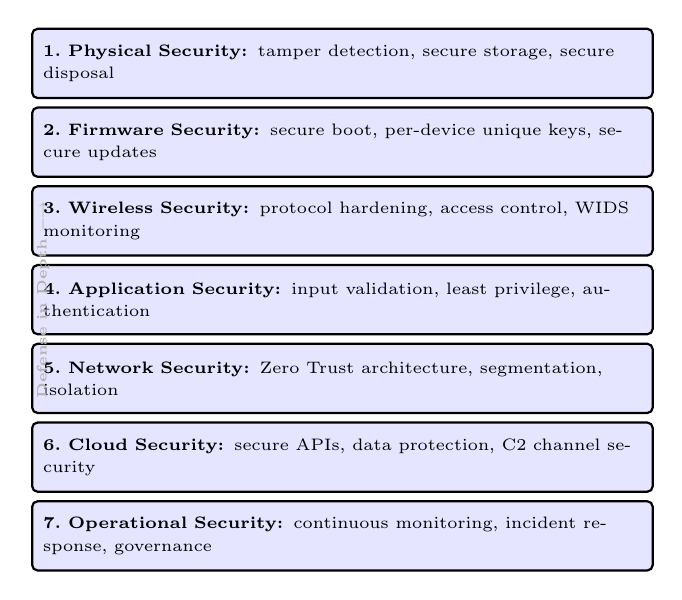
\begin{tikzpicture}[
  font=\fontsize{6.5pt}{8pt}\selectfont,
  >=Stealth,
  cbar/.style={
    rectangle, rounded corners=2pt, draw, thick,
    minimum width=7.8cm, minimum height=0.88cm,
    align=left, text width=7.6cm, inner sep=4pt,
    fill=blue!10
  }
]
  \node[cbar] at (0, 0.00)
    {\textbf{1.\ Physical Security:} tamper detection, secure storage, secure disposal};
  \node[cbar] at (0,-1.00)
    {\textbf{2.\ Firmware Security:} secure boot, per-device unique keys, secure updates};
  \node[cbar] at (0,-2.00)
    {\textbf{3.\ Wireless Security:} protocol hardening, access control, WIDS monitoring};
  \node[cbar] at (0,-3.00)
    {\textbf{4.\ Application Security:} input validation, least privilege, authentication};
  \node[cbar] at (0,-4.00)
    {\textbf{5.\ Network Security:} Zero Trust architecture, segmentation, isolation};
  \node[cbar] at (0,-5.00)
    {\textbf{6.\ Cloud Security:} secure APIs, data protection, C2 channel security};
  \node[cbar] at (0,-6.00)
    {\textbf{7.\ Operational Security:} continuous monitoring, incident response, governance};

  %% Left-edge bracket label (no overflow — stays inside bar region)
  \node[font=\fontsize{5.5pt}{7pt}\selectfont\bfseries, text=gray!60,
        rotate=90, anchor=south]
    at (-3.6,-3.00) {Defense in Depth $\longrightarrow$};

\end{tikzpicture}
\caption{Seven-layer defense-in-depth security framework for robotic systems.
  Each layer provides independent controls so that a vulnerability at one layer
  does not lead to complete system compromise.}
\label{fig:defense_framework}
\end{figure}

\section{Implementation Recommendations}

\textbf{Deploying Organizations}: Conduct pre-deployment security assessment with
third-party penetration testing; segment robot networks from critical systems; establish
behavioral monitoring baselines; maintain robot-specific incident response plans; patch
promptly when vulnerabilities are disclosed.

\textbf{Manufacturers}: Never use hardcoded credentials; provision per-device unique
identities during manufacturing; implement secure boot with hardware roots of trust;
maintain coordinated vulnerability disclosure programs; commit to security updates for
minimum 5--10 year product lifetimes.

\textbf{Policymakers}: Establish mandatory baseline security standards and certification
for critical infrastructure robotics; clarify manufacturer and operator liability; mandate
incident reporting; fund robotics security research and specialist training.

\section{Conclusion}

The UniPwn wormable exploit affecting Unitree robots demonstrates the catastrophic
potential when fundamental security vulnerabilities converge in autonomous systems with
physical-world interaction capabilities. For critical infrastructure organizations,
compromised robots represent trusted insiders with physical access, legitimate credentials,
and kinetic capabilities enabling weaponization against the infrastructure they were
designed to protect.

Addressing these challenges requires the seven-layer defense-in-depth framework proposed
here: eliminating hardcoded credentials through per-device cryptographic identities;
implementing secure boot with hardware roots of trust; hardening wireless protocols with
mutual authentication; validating inputs against command injection; applying Zero Trust
micro-segmentation; securing cloud management channels; and maintaining continuous
behavioral monitoring with rapid incident response.

The robot zombie apocalypse scenario reflects genuine operational risk as dependence on
autonomous systems for critical functions grows. The convergence of mobility, wireless
connectivity, physical interaction, and autonomy creates threat potential exceeding
traditional cybersecurity concerns. The age of autonomous robotics has arrived; the age
of secure autonomous robotics must follow.

\bibliographystyle{IEEEtran}
\begin{thebibliography}{20}

\bibitem{udinmwen2025calm}
E. Udinmwen, ``Calm Down Everyone---Unitree's Recently Discovered Exploit,'' \textit{TechRadar Pro}, Oct.~2025.

\bibitem{naraine2025hackers}
R. Naraine, ``Hackers Could Unleash Chaos Through Backdoor in China-Made Robot Dogs,'' \textit{SecurityWeek}, Apr.~2025.

\bibitem{gosavi2025unitree}
A. Gosavi, ``Unitree Humanoid Robots Send Data to China Every 5 Minutes,'' \textit{Interesting Engineering}, Oct.~2025.

\bibitem{antonakakis2017understanding}
M. Antonakakis et al., ``Understanding the Mirai Botnet,'' in \textit{Proc.\ 26th USENIX Security Symp.}, Aug.~2017, pp.~1093--1110.

\bibitem{weaver2003very}
N. Weaver, V. Paxson, S. Staniford, and R. Cunningham, ``A Taxonomy of Computer Worms,'' in \textit{Proc.\ ACM WORM}, Oct.~2003, pp.~11--18.

\bibitem{costin2014large}
A. Costin, J. Zaddach, A. Francillon, and D. Balzarotti, ``A Large-Scale Analysis of the Security of Embedded Firmwares,'' in \textit{Proc.\ 23rd USENIX Security Symp.}, Aug.~2014, pp.~95--110.

\bibitem{murphy2019robotics}
R.~R. Murphy, K.~L. Decker, and J.~A. Adams, ``Robotics in Critical Infrastructure,'' in \textit{Springer Handbook of Robotics}. Springer, 2019, pp.~1981--2004.

\bibitem{checkoway2011comprehensive}
S. Checkoway et al., ``Comprehensive Experimental Analyses of Automotive Attack Surfaces,'' in \textit{Proc.\ 20th USENIX Security Symp.}, Aug.~2011, pp.~447--462.

\bibitem{ronen2017iot}
E. Ronen, A. Shamir, A.-O. Weingarten, and C. O'Flynn, ``IoT Goes Nuclear,'' in \textit{Proc.\ IEEE S\&P}, May~2017, pp.~195--212.

\bibitem{petit2015remote}
J. Petit and S.~E. Shladover, ``Potential Cyberattacks on Automated Vehicles,'' \textit{IEEE Trans.\ Intell.\ Transp.\ Syst.}, vol.~16, no.~2, pp.~546--556, 2015.

\bibitem{eykholt2018robust}
K. Eykholt et al., ``Robust Physical-World Attacks on Deep Learning,'' in \textit{Proc.\ CVPR}, June~2018, pp.~1625--1634.

\bibitem{gu2017badnets}
T. Gu, B. Dolan-Gavitt, and S. Garg, ``BadNets,'' arXiv:1708.06733, Aug.~2017.

\bibitem{yaacoub2020cyber}
J.-P.~A. Yaacoub et al., ``Robotics Cyber Security,'' \textit{Int.\ J.\ Inf.\ Security}, vol.~21, pp.~115--158, 2022.

\bibitem{alemzadeh2016targeted}
H. Alemzadeh et al., ``Targeted Attacks on Teleoperated Surgical Robots,'' in \textit{Proc.\ DSN}, June~2016, pp.~395--406.

\bibitem{iec62443}
IEC, ``IEC 62443 Series: Industrial Network and System Security,'' Geneva, 2018.

\bibitem{nist800160}
R. Ross, M. McEvilley, and J.~C. Oren, ``Systems Security Engineering,'' NIST SP~800-160 Vol.~1, Nov.~2016.

\bibitem{cisa2023ics}
CISA, ``Recommended Practice: Developing an ICS Cybersecurity Incident Response Capability,'' Oct.~2023.

\bibitem{wu2016survey}
M. Wu et al., ``A Survey of Cyber Attacks on Cyber Physical Systems,'' \textit{IEEE/CAA J.\ Autom.\ Sin.}, vol.~4, no.~2, pp.~176--193, 2017.

\end{thebibliography}

\end{document}
